\section{Microservice Architecture}
\label{se:microservice}

A microservice architecture style is an approach to developing a single application as a package of small services, each working in their own process and communicating with lightweight mechanisms, often through the delivery of \hl{a RESTful API}. These services are built around commercial capacities and can be used independently by fully automated implementation machines \cite{LewisMicroservices}. \hl{These services are implemented independently with minimizing the centralized dependencies. Thus each microservice may be written in different programming languages and use different data storage technologies}.

% \hl{Among the characteristics of microservice, a few characteristics heavily affect while moving from} \acrshort{soa} to microservice.
There are lots of microservice patterns developed and evolved. Throughout the following sections, we will discuss in brief some of the microservice design patterns mostly used in the context of designing \acrshort{wdias} architecture. Next, we will discuss how microservice architecture promote to only to create endpoints which only belong to each service logical domain. Next, discuss only using database per service which allows to loosely couple between systems and achieves high scalability. In Sagas, we discuss how distributed transactions can achieve over microservices. Next, we will discuss a concept called \emph{the scale cube}, which explains the scalability from the perspective of x,y, and z-axis.


%%%%%%%%%%%%%%%%%%%%%%%%%%%%%%%%%%%%%%%%%%%%%%%%%%%%%%%%%%%%%%%%%%%%%%%%%%%%%%%%
\subsection{Smart Endpoints and Dumb Pipes}
\label{subse:dumb_pipes}
\dbc{At the end of previous para tell what will be discussed in the next set of sub-section. A single sentence like "Next, we will discusss ...." is enough}
\gkc{FIXED}

When building communication endpoints, \hl{many architectural approaches are adding significant smart by providing different protocol supports and complex logic support via the endpoints.} As an example \acrshort{esb} support multiple protocols and endpoints can use complex logic. But microservice architecture follows an alternative approach called as \emph{Smart endpoints and dumb pipes} \cite{LewisMicroservicesPipes}.
Applications built on the basis of microservices are intended to be as disconnected and as coherent as possible. They have their domain logic and work more like filters in the classical Unix meaning. After receiving a request, apply the correct logic and produce a response. And it uses simple RESTful protocols instead of complex protocols.
\dbc{RESTish or RESTful?}
\gkc{Yes. Changed.}

%%%%%%%%%%%%%%%%%%%%%%%%%%%%%%%%%%%%%%%%%%%%%%%%%%%%%%%%%%%%%%%%%%%%%%%%%%%%%%%%
\subsection{\hl{Database per Microservice}}
\label{subse:database_per_service}

\acrshort{microservice} prefers to have each service manage its database, either different instances of the same database technology or entirely different database systems - an approach called \emph{Polyglot Persistence} \cite{LewisMicroservicesManagement}.

The idea is to keep the persistent data of each microservice private for this service and only to make it accessible via the \acrshort{api}.
There are different ways to keep the permanent data of a service private. It is not necessary to set up a database server for each service. For example, when you use a relational database, the following methods can be used to keep the data private. \cite{RichardsonMicroservicesService}:
\begin{itemize}
    \item \emph{Private tables per service} –- each service has a set of tables that this service should not have access to.
    \item \emph{Schema per service} –- each service has a private database schedule for this service.
    \item \emph{Database server per service} -– each service has its database server.
\end{itemize}
\emph{private tables per service} and \emph{schedule per service} have the lowest overhead. The use of an \emph{schedule per service} is interesting because it makes the property clearer. Some high throughput services may require their database server.

%%%%%%%%%%%%%%%%%%%%%%%%%%%%%%%%%%%%%%%%%%%%%%%%%%%%%%%%%%%%%%%%%%%%%%%%%%%%%%%%
\subsection{\hl{Distributed Transactions over Microservices}}
\label{subse:sagas}
To guarantee a loose coupling, every microservice can have its own database. Maintaining data consistency between services is a challenge because 2 phase-commit/distribution transactions are not an option for many applications. A service publishes an event when the data changes. Other services use this event and update their data \cite{RichardsonMicroservicesSagas}. This is also called the \emph{Saga pattern}.

%%%%%%%%%%%%%%%%%%%%%%%%%%%%%%%%%%%%%%%%%%%%%%%%%%%%%%%%%%%%%%%%%%%%%%%%%%%%%%%%
\subsection{\hl{Concept of Scale Cube}}
\label{subse:scale_cube}
\gkc{I can not think about any other title than this.}
The scalability of a system can explain via a concept called \emph{Scale Cube} which talks about the scalability of the application by defining over X, Y and Z axis.

\paragraph{X-axis Scaling}-- When scaling the X-axis, multiple instances of an application execute behind a load balancer. If there are \textit{n} copies then each copy handles 1/\textit{n} of the load. A commonly used simple approach to scaling a service.

\paragraph{Y-axis Scaling}-- When compared to the Z-axis and X-axis scaling, which follows the concept of running multiple identical copies of the application, but Y-axis axis scaling segregate the application into multiple services in same domain. So, the end services are responsible for one or more closely related functions. There are different ways to split the application into services.
\begin{itemize}
    \item verb-based decomposition. e.g., checkout.
    \item decompose the application by noun. e.g., order management. 
    \item it possible to use a combination of verb-based and noun-based decomposition for an application.
\end{itemize}

\emph{The microservice architecture is an application of Y-axis scaling}.

\paragraph{Z-axis Scaling}-- The Z-axis scaling is following the concept of each service runs an same application code (similar to X-axis scaling). The big difference is that each service is responsible for only a subset of the data. 
Z-axis splits are commonly used to scale databases. Data is partitioned (a.k.a. sharded) across a set of servers based on an attribute of each record.

Even \acrshort{wdias} is a design based on the Y-axis scaling, it is possible to use the Z-axis scaling to scaling the system further. This will be more discussion in \cref{se:discussion}.


%%%%%%%%%%%%%%%%%%%%%%%%%%%%%%%%%%%%%%%%%%%%%%%%%%%%%%%%%%%%%%%%%%%%%%%%%%%%%%%%
% \subsection{Brief introduction to the \acrfull{k8s}}
% \label{sebse:k8s_intro}
\dbc{Don't present this as a separate section. Either this need to be in the literature survey, or integrate key ideas into another section as a paragraph.}
\gkc{Move this as a paragraph at the end of the architectural decisions}


%%%%%%%%%%%%%%%%%%%%%%%%%%%%%%%%%%%%%%%%%%%%%%%%%%%%%%%%%%%%%%%%%%%%%%%%%%%%%%%%
\subsection{\acrshort{wdias} Microservices}
\label{sebse:wdias_microservices}
As seen in Figure of \cref{fi:wdias_micro_on_demand} and \cref{fi:wdias_micro_async} each circle represents a microservice in the \acrshort{wdias}, and those are implemented as containerized applications.
\begin{figure}[htp]
    \centering
    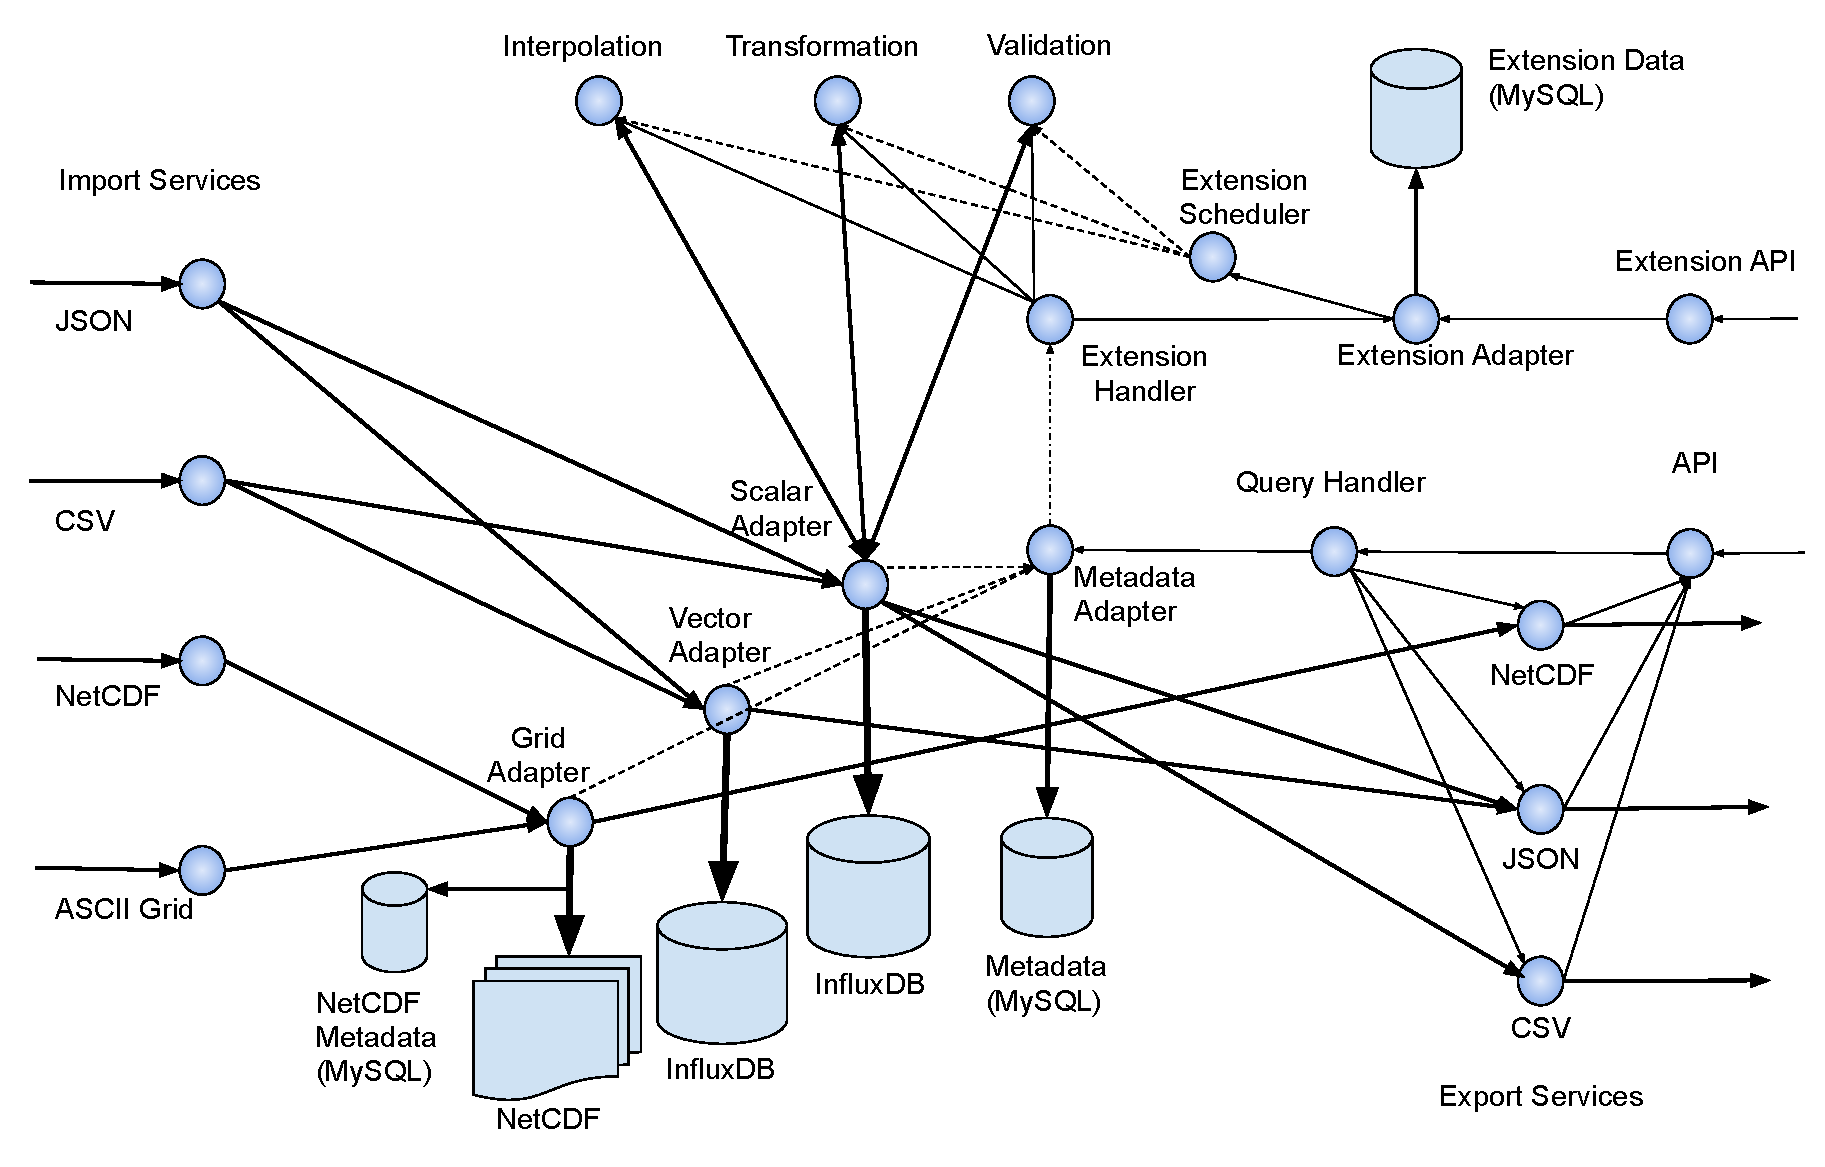
\includegraphics[width=1\textwidth]{method/microservice/microservice_architecture-handle_on_demand-v4.pdf}
    \caption{\acrshort{wdias} architecture for handling requests on demand}
    \label{fi:wdias_micro_on_demand}
\end{figure}
The left side of \cref{fi:wdias_micro_on_demand} shows the import modules of the \acrshort{wdias}, and the right side shows the export modules. As explained section \cref{subse:dumb_pipes}, each import microservice only does the specific task of converting and forwarding the request to the correct data adapter module.
For each data type, there is an adapter microservice is running which is optimized to storing such type of data. And the metadata data of the timeseries store using \acrshort{rdbms} which gives more performance over retrieving metadata data. The metadata is cached with the In-Memory database to fast access as mentioned in \cref{subse:redis}.
The system generates a unique identifier for each timeseries, and throughout the \acrshort{wdias}, other microservice use it to handle data for fast access.

\begin{figure}[htp]
    \centering
    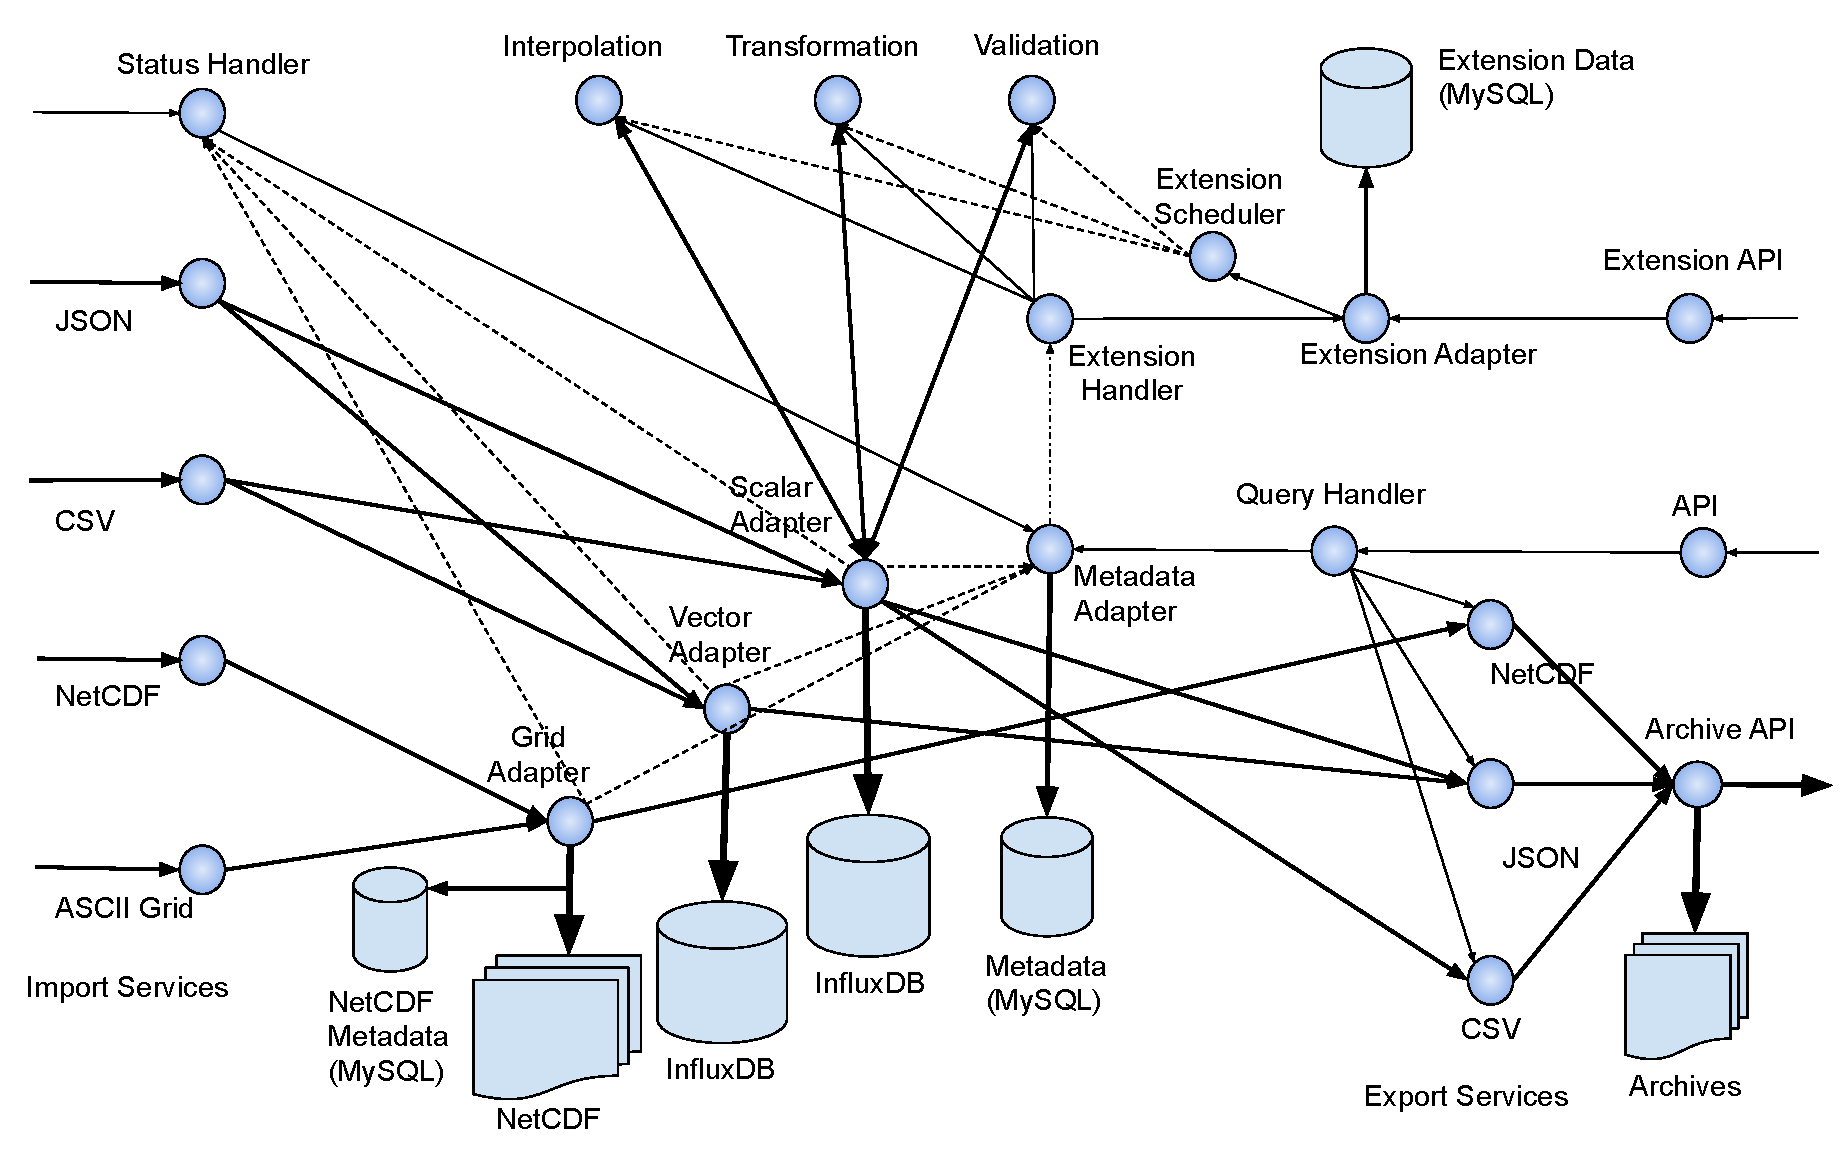
\includegraphics[width=1\textwidth]{method/microservice/microservice_architecture-handle_on_async-v4.pdf}
    \caption{\acrshort{wdias} architecture for handling requests asynchronously.}
    \label{fi:wdias_micro_async}
\end{figure}
Export module microservice follows the same concepts and provides the capability to export the data into required formats of the weather models. Each adapter follows the concept of database per service as mentioned in \cref{subse:database_per_service}. This gives the freedom for \acrshort{wdias} to scale better with \acrshort{k8s}.

As shown in \cref{fi:wdias_micro_on_demand}, when a smaller size request comes to the system, it handles on-demand and response back. However, as shown in \cref{fi:wdias_micro_async}, when a request with a larger size comes to the system, it stores the data for asynchronously process the data and responds with a unique id that can use to verify whether data processed successfully or not. Here is uses the microservice concept of Saga as mentioned in \cref{subse:sagas} while processing the Grid data. First, it stores the data and responds to the user. Then publish an event, and another service listens to those events and process the data and update the system status.

\begin{figure}[htp]
    \centering
    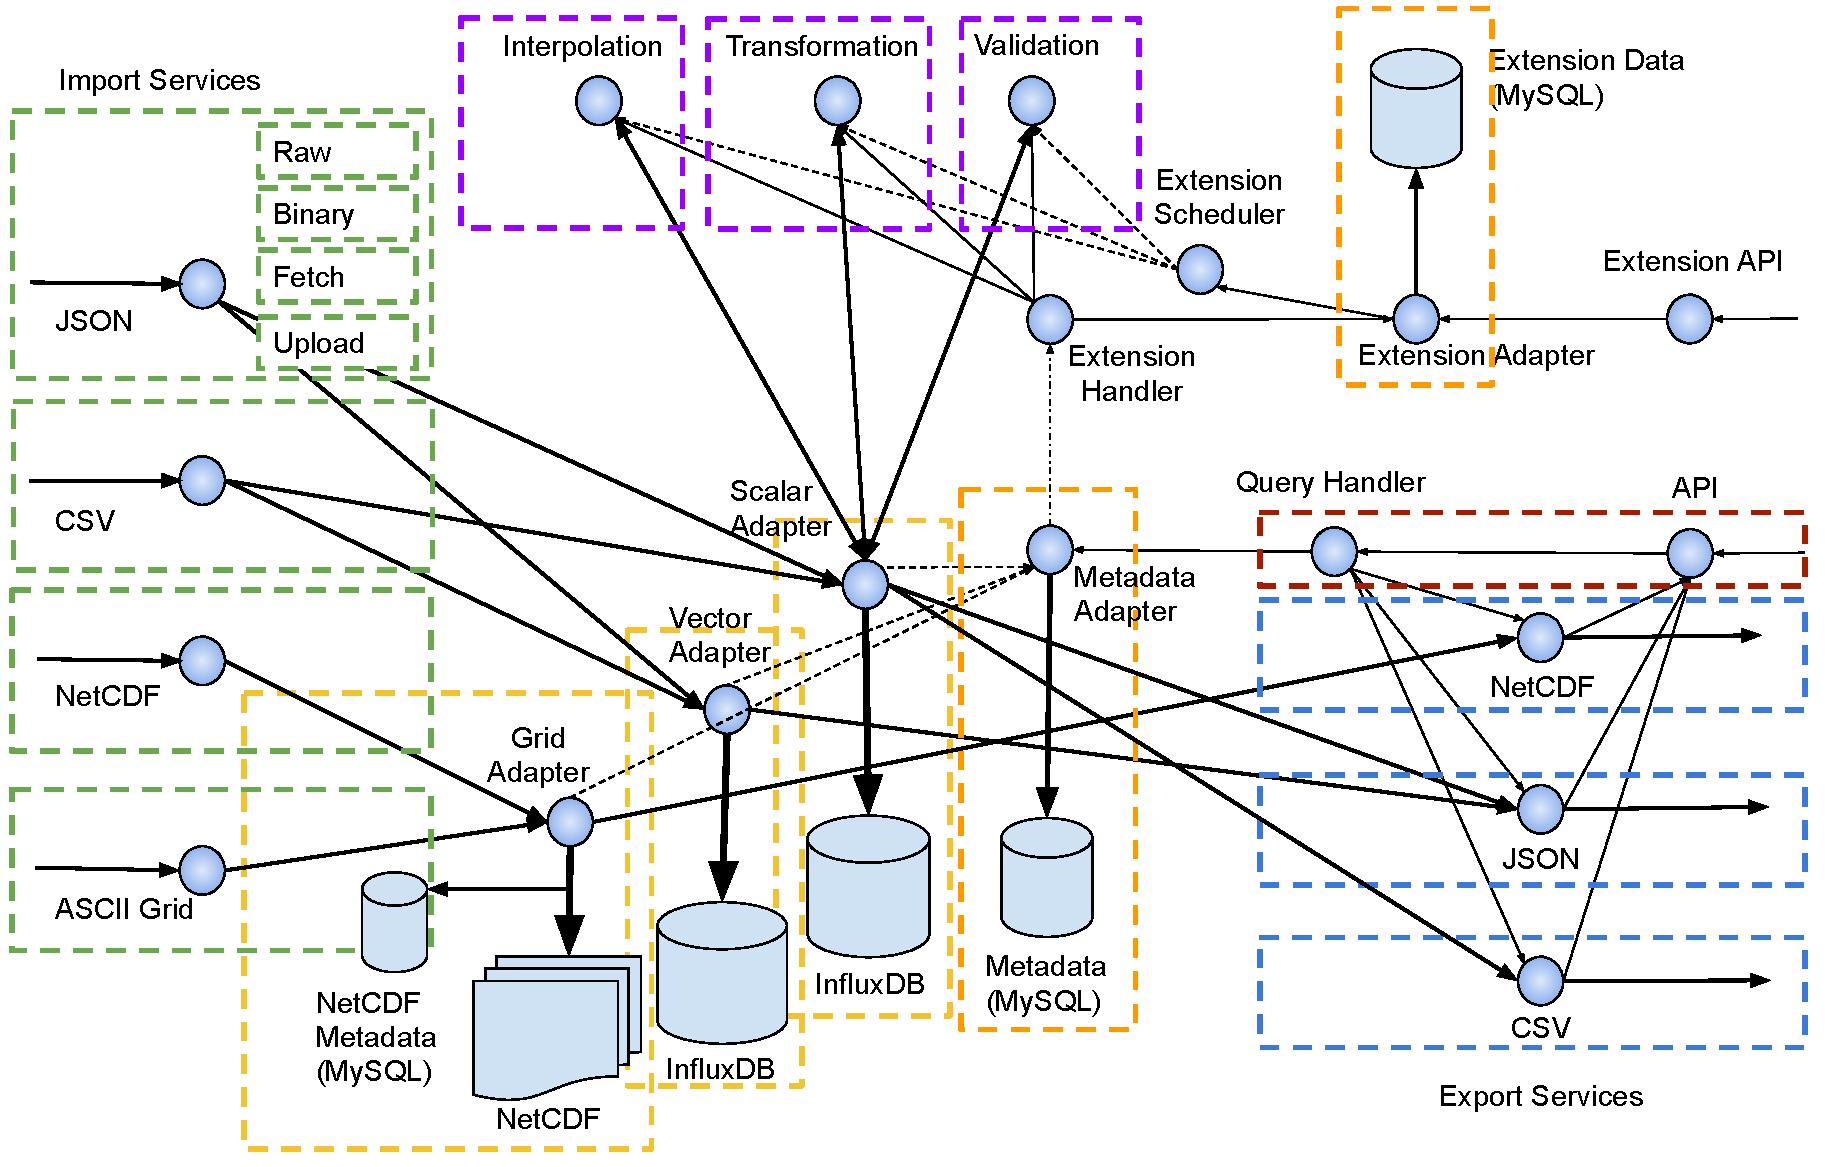
\includegraphics[width=1\textwidth]{method/microservice/separation_microservices-v4.pdf}
    \caption{Separation of \acrshort{wdias} microservices.}
    \label{fi:wdias_micro_separation}
\end{figure}
\cref{fi:wdias_micro_separation} shows the clear separation of microservices into the modules of the \acrshort{wdias}. As shown, each adapter has an isolated database, and the database is hosted separately for the high performance. 
Apart from that, as we further discuss in \cref{se:data_preprocess}, the extension modules are running separately such as Interpolation, Transformation, and Validation, etc. 
The Extension Adapter allows users to register new triggers for the extensions. And extension scheduler triggers the events based on time and extension handler triggers event based on data change.


%%%%%%%%%%%%%%%%%%%%%%%%%%%%%%%%%%%%%%%%%%%%%%%%%%%%%%%%%%%%%%%%%%%%%%%%%%%%%%%%
\subsection{\acrshort{wdias} \acrfull{api}}
\label{sebse:wdias_api}
One of the main design considerations in \acrshort{wdias} is the convention of defining the \acrshort{api}. It follows a simple RESTful \acrshort{api}, and allow users to interact with HTTP methods.

\emph{Timeseries} endpoints allow users to interact with Metadata Adapter, and those are cache on the Query Handler to perform search queries. These are the main endpoints to handle timeseries metadata which defines unique timeseries identifier based on the metadata values. As an example, if it needs to extend the system to store irregular grid data, then it should add another set of location endpoints for storing irregular grid location details.
\begin{itemize}
    \item parameter
    \begin{itemize}
        \item \texttt{GET /parameter} -- Get parameters
        \item \texttt{POST /parameter} -- Create parameter
        \item \texttt{PUT /parameter/id} -- Update parameter
        \item \texttt{DELETE /parameter/id} -- Delete parameter
    \end{itemize}
    \item timeStep
    \begin{itemize}
        \item \texttt{GET /timestep} -- Get TimeSteps
        \item \texttt{POST /timestep} -- Create TimeStep
        \item \texttt{PUT /timestep/id} -- Update TimeStep
        \item \texttt{DELETE /timestep/id} -- Delete TimeStep
    \end{itemize}
\dbc{Format others as above}
\gkc{FIXED}
    \item location
    \begin{itemize}
        \item \texttt{GET /location} -- Get location points
        \item \texttt{POST /location} -- Create location point
        \item \texttt{PUT /location/id} -- Update location point
        \item \texttt{DELETE /location/id} -- Delete location point
        \item \texttt{GET /location/regular-grid} -- Get regular grids
        \item \texttt{POST /location/regular-grid} -- Create regular grid
        \item \texttt{PUT /location/regular-grid/id} -- Update regular grid
        \item \texttt{DELETE /location/regular-grid/id} -- Delete regular grid
    \end{itemize}
    \item timeseries
    \begin{itemize}
        \item \texttt{GET /timeseries} -- Get timeseries
        \item \texttt{POST /timeseries} -- Create timeseries
        \item \texttt{PUT /timeseries/id} -- Update timeseries
        \item \texttt{DELETE /timeseries/id} -- Delete timeseries
    \end{itemize}
\end{itemize}

\emph{Import} endpoints allow to upload data into the \acrshort{wdias} system.
\begin{itemize}
    \item \texttt{POST /import/json/raw} -- Insert Scalar/Vector timeseries data with JSON body
    \item \texttt{POST /import/csv/raw} -- Insert Scalar/Vector timeseries data in CSV format
    \item \texttt{POST /import/ascii-grid/upload} -- Upload set of ASCII Grid files
    \item \texttt{POST /import/ascii-grid/binary} -- Upload a single ASCII Grid file
\end{itemize}

\emph{Export} endpoints allow to get/download data from the \acrshort{wdias} system.
\begin{itemize}
    \item \texttt{GET /export/json/raw} -- Get Scalar/Vector timeseries data in JSON format
    \item \texttt{GET /export/json/raw?start=2000-01-01\&end=2000-01-03} -- Get Scalar/Vector timeseries data in JSON format for given time period
    \item \texttt{GET /export/netcdf/binary} -- Download Grid data timeseries data in \acrshort{netCDF} format
\end{itemize}

\emph{Extensions} endpoints for configure extensions. These details describes in the \cref{se:data_preprocess}.

As mentioned above, other than the timeseries metadata which is the core of the data system, other module endpoints start with the module name such as import, export, and extension. This allows adding a new module system if required. 
For import and export modules, then follows by the data format. This provides the flexibility to integrate new data format modules. 
Then the endpoint name ends with the data upload/insert data type. Data can upload as a single file with binary or multiple files with the upload. Or in the body of the request as raw, and need to send the required headers has mentioned by a particular module.
Thus the \acrshort{api} convention of \texttt{\hl{/MODULE/DATA\_FORMAT/DATA\_TYPE}} allows users to integrate new import or export modules into the system as well as add new data types.
